\section{\NP{} as puzzles, or one-move games}

Recall that \NP{} is the class of problems solvable by guess-and-check, with a
\emph{check} problem in \P{} (\cref{def:np}):
\[
  \NP = \SetBuilder{L}{
    ∃\underbrace{\mathstrut L'∈\P}_{\mathclap{\text{the ``check'' problem}}} \;
    ∀x \quad
    x∈L ⟺ \underbrace{∃g \; (x, g) ∈ L'}_{\mathclap{\text{guess-and-check}}}
  }.
\]
(In the above, it is \emph{implicitly} required that \(\Abs g\) be
polynomially-bounded with respect to \(\Abs x\), but we have omitted it in
notation for readability.)

Another famous example of a problem in \NP{} is Sudoku, framed as the following
decision problem:
\begin{definition}[\Problem{sudoku}]%
  We are given a square grid with dimensions \(n^2\times n^2\), some of whose
  cells are filled in with numbers in \(\{1,\dotsc,n^2\}\).  Call this grid the
  Sudoku \emph{board}.  The board is evenly partitioned into \(n\) chunks along
  each axis, resulting in \(n^2\) \emph{blocks} each with dimensions \(n\times
  n\).

  Does there exist a way to fill in the rest of the cells so that each row,
  column, and block on the filled-in board contains each number in
  \(\{1,\dotsc,n^2\}\) exactly once?
\end{definition}

\begin{center}
  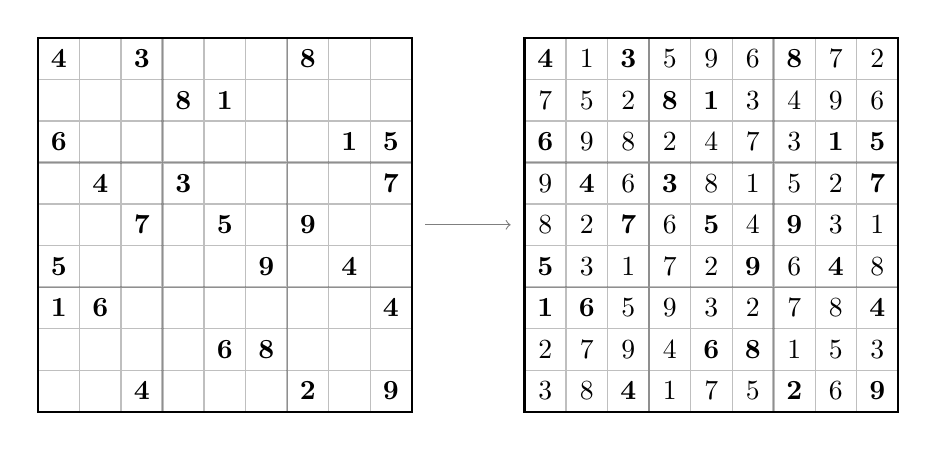
\begin{tikzpicture}[x=3em/2, y=3em/2]
    \tikzset{
      sudoku/.pic={
        \draw[thick] (0,0) rectangle (9,-9);
        \draw[thick, opacity=1/4]
        foreach \i in {3,6} { (0,-\i) -- +(9,0) (\i,0) -- +(0,-9) };
        \draw[opacity=1/4]
        foreach \i in {1,...,8} { (0,-\i) -- +(9,0) (\i,0) -- +(0,-9) };

        \path
        foreach \i in {0,...,8} { foreach \j in {0,...,8} {
            (\j+1/2,-\i-1/2) coordinate(#1-\i-\j)
        } }
        foreach \i/\j/\val in {
          0/0/4,0/2/3,0/6/8,
          1/3/8,1/4/1,
          2/0/6,2/7/1,2/8/5,
          3/1/4,3/3/3,3/8/7,
          4/2/7,4/4/5,4/6/9,
          5/0/5,5/5/9,5/7/4,
          6/0/1,6/1/6,6/8/4,
          7/4/6,7/5/8,
          8/2/4,8/6/2,8/8/9
        } { (#1-\i-\j) node{\(\mathbf\val\)} }
        foreach \i/\j/\name in {4.5/0/w,4.5/9/e} {
          (\j,-\i) coordinate(#1-\name)
        };
      },
    }


    \matrix[column sep=4em]{
      \pic{sudoku=a}; & \pic{sudoku=b}; \\
    };
    \draw[opacity=1/2, arrows={_[sep=1em/2]-To[sep=1em/2]}] (a-e) -- (b-w);

    \path
    foreach \i/\j/\val in {
      0/1/1,0/3/5,0/4/9,0/5/6,0/7/7,0/8/2,
      1/0/7,1/1/5,1/2/2,1/5/3,1/6/4,1/7/9,1/8/6,
      2/1/9,2/2/8,2/3/2,2/4/4,2/5/7,2/6/3,
      3/0/9,3/2/6,3/4/8,3/5/1,3/6/5,3/7/2,
      4/0/8,4/1/2,4/3/6,4/5/4,4/7/3,4/8/1,
      5/1/3,5/2/1,5/3/7,5/4/2,5/6/6,5/8/8,
      6/2/5,6/3/9,6/4/3,6/5/2,6/6/7,6/7/8,
      7/0/2,7/1/7,7/2/9,7/3/4,7/6/1,7/7/5,7/8/3,
      8/0/3,8/1/8,8/3/1,8/4/7,8/5/5,8/7/6
    } { (b-\i-\j) node{\(\val\)} };
  \end{tikzpicture}
\end{center}

For this problem, a ``guess'' \(g\) consists of a list of numbers in
\(\{1,\dotsc,n^2\}\) specifying the values with which to fill in the empty
cells in the given grid.  Then, the ``check'' problem \(L'\) is stated as
follows:
\begin{nested}
  Given a fully-filled-in Sudoku board, does each row, column, and block on the
  grid contain each of \(\{1,\dotsc,n^2\}\) exactly once?
\end{nested}

Sudoku, being a natural puzzle, illustrates how any problem in \NP{} can be
thought of as a one-player ``game'' consisting of one turn, played on a given
input \(x\) (e.g., the Sudoku board), in which the player makes a move by
writing down a guess \(g\) (e.g., the filled-in values), then wins if,
according to the rules of the game, \((x, g) \in L'\) (e.g., the filled-in
board meets the Sudoku conditions).  The decision problem can now be stated as
the question, \emph{does the player have a winning strategy?}

%Also recall an example of an \NP{} problem, \Problem{hamiltonian-path}
%(\cref{def:hamiltonian-path}), which asks: given a graph, does it have a
%Hamiltonian path?  Here, the ``check'' problem \(L'\) can be stated as follows:
%\begin{nested}
%  Given a graph \(x = \Gamma\) with vertices \(v_1,\dotsc,v_n\), along with a
%  permutation \(g = \phi(1),\dotsc,\phi(n)\), does the sequence
%  \(v_{\phi(1)},\dotsc,v_{\phi(n)}\) specify a valid path on \(\Gamma\)?
%\end{nested}
%
%We can now intuitively reframe \Problem{hamiltonian-path} as a one-player
%``game'', played on an input ``board'' in the form

%in which the player writes down some
%permutation \(\phi\).  They ``win'' if it meets the validity condition \((x, g)
%\in L'\) and ``lose'' if it doesn't.  Under this framing, the decision problem
%becomes the following question: does the player have a winning \emph{strategy}?


